%=============================--A--=============================%
\newpage
\section{Peculiaridades}
\label{sec:peculiaridades}
De modo a manter a discussão o mais sucinta possível, serão abordados nesta secção conceitos \textbf{fulcrais} da implementação que não serão mencionados posteriormente, por questões de brevidade. Salienta-se a necessidade primordial de expor estes conceitos antes da análise do esquema desenvolvido. 
%1
%1
%=============================--B--=============================%
\subsection{1. Transition width}
\label{subsec:transition-width}
\textbf{Definição:} diferença entre a frequência em que a \textit{stopband} começa (aproximadamente, por volta dos $-60$ dB) e a frequência em que o sinal começa a ser rejeitado (i.e., quando a \textit{passband} termina; na periferia dos $-6$ dB), relativamente às frequências de corte dos filtros.

%\iffalse
\begin{figure}[H]
    \centering
    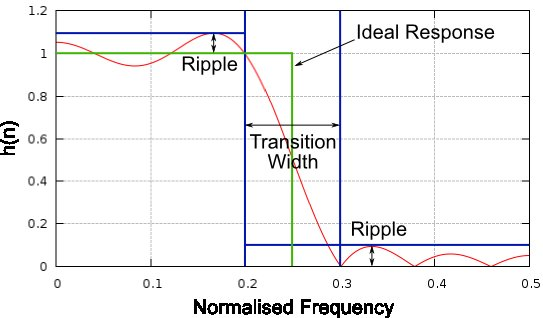
\includegraphics[width = 0.7\linewidth]{img/transition-width.png}
    \caption{Exemplo da representação da \textit{transition width} de um filtro de processamento de sinal.}
    \label{fig:transition-width}
\end{figure}
%\fi

Na elaboração do laboratório, com o uso do \textit{software} GNU Radio, foram somente utilizados filtros FIR (\textit{finite impulse response}), que apresentam uma relação entre a \hyperref[subsec:transition-width]{subsecção em discussão} e a \hyperref[subsec:delay]{seguinte}:

% https://lists.gnu.org/archive/html/discuss-gnuradio/2017-11/msg00018.html
\textit{"(...) If you use a FIR filter and use a small transition width, processing speed of the program will degrade, as more filter taps are needed. If you use a large transition width, the speed of the program improves (less taps are needed), but you have to deal with the lousy frequency response of the filter. (...)"}\cite{fwd:transitionwidth}

Fator delimitado com base nestes \textit{trade-offs} verificados empiricamente.
\newline\break
\noindent\fcolorbox{black}{white}{%
    \minipage[t]{\dimexpr\linewidth-2\fboxsep-2\fboxrule\relax}
        \textbf{Observações} $\rightarrow$ Para valores ínfimos deste parâmetro, verificou-se uma perda de informação indesejável do sinal. No espectro oposto, para elevados valores de transição, foi constatada uma captação de informação não solicitada (apesar de atenuada; vide a \hyperref[fig:transition-width]{imagem acima}) e maior prevalência de ruído.
    \endminipage}
\newline\break
Foi admitida uma \textit{transition width} de $1$ kHz na maioria dos filtros implementados, nomeadamente do \hyperref[subsec:mod3]{módulo 3} (\textit{trade-off} entre delay e ruído, como veremos \hyperref[subsec:delay]{em seguida}), com exceção dos filtros passa-baixo finais com uma largura de transição diminuta de $200$ Hz (a motivação para esta modificação foi a aniquilação de perturbações sonóras, derivadas do ruído, experienciadas).
%2
%2
%=============================--C--=============================%
\subsection{2. Delay}
\label{subsec:delay}
\textbf{Definição:} denominamos por \textit{group delay} o atraso em número inteiro de amostras, incutido pela utilização única, ao longo do projeto, de filtros do tipo \textit{"Decimating FIR filter"}, com resposta em fase linear. \\ \textit{Group delay}\cite{jayesparmarja} $\delequal K = (N-1)/2$, em que $N$ representa o número de \textit{taps} do filtro. Para obter o atraso temporal, naturalmente se deduz que: \\ \textit{Time delay}\cite{jayesparmarja} $\delequal K = (N-1)/2\text{F}_\text{S}$, onde $\text{F}_\text{S}$ denomina a frequência de amostragem (\textit{sample rate}).
\newline\break
\noindent\fcolorbox{black}{white}{%
    \minipage[t]{\dimexpr\linewidth-2\fboxsep-2\fboxrule\relax}
        \textbf{Observações} $\rightarrow$ Com o aumento da \textit{sample rate} verifica-se uma diminuição do \textit{delay} temporal.
        O \textit{group delay} aumenta linearmente com o número de \textit{taps} do filtro.
    \endminipage}
\newline\break

Dado que o \textit{source code} do \textit{software} GNU Radio utilizado se encontra disponível (distribuído sobre os termos da licença GPL e \textit{copyrighted} pela Free Software Foundation), foi efetuada uma análise sucinta que se traduziu em ilações bastante curiosas.

\begin{lstlisting}[caption=\textit{Source code}: \color{white}{\underline{https://github.com/gnuradio/gnuradio/blob/master/gr-filter/lib/firdes.cc}}, frame=tlrb]{saucecode}
int firdes::compute_ntaps_windes(
    double sampling_freq,
    double transition_width, // this is frequency, not relative frequency
    double attenuation_dB)
{
    // Based on formula from Multirate Signal Processing for
    // Communications Systems, fredric j harris
    int ntaps = (int)(attenuation_dB * sampling_freq / (22.0 * transition_width));
    if ((ntaps & 1) == 0) // if even...
        ntaps++;          // ...make odd
    return ntaps;
}

int firdes::compute_ntaps(double sampling_freq,
                          double transition_width,
                          fft::window::win_type window_type,
                          double param)
{
    double a = fft::window::max_attenuation(window_type, param);
    int ntaps = (int)(a * sampling_freq / (22.0 * transition_width));
    if ((ntaps & 1) == 0) // if even...
        ntaps++;          // ...make odd

    return ntaps;
}
\end{lstlisting}

É diretamente observado que o número de \textit{taps} é inversamente proporcional à \textit{transition width}, i.e., uma menor \textit{transition width} traduz-se num maior \textit{delay}. Fica então corroborada a relação íntima entre \hyperref[subsec:delay]{esta subsecção} com \hyperref[subsec:transition-width]{a anterior}, como supramencionado. 

Verifica-se que para uma dada frequência de corte, uma \textit{transition width} menor, corresponde a uma \textit{roll-off slope} mais acentuada (maior ordem do filtro, no sentido familiar analógico). Pelo que o número de \textit{taps} representa a ordem do filtro. É então de fácil entendimento a degradação do tempo de processamento do programa com o incremento do número de \textit{taps}.

Outro aspecto a salientar é o facto do número de \textit{taps} se encontrar diretamente proporcional à \textit{sample rate}, o que reporta o melhor funcionamento dos filtros utilizados a altas frequências de amostragem.
\newline\break
\noindent\fcolorbox{black}{white}{%
    \minipage[t]{\dimexpr\linewidth-2\fboxsep-2\fboxrule\relax}
        \textbf{Observações} $\rightarrow$ Para os parâmetros projetados (\textit{transition width} e \textit{sample rate}), o \textit{delay} que compensa o atraso induzido no ramo que efetua a recuperação de $L - R$ (dado que apresenta o maior número de filtragens) é de 25 \textit{samples}. A localização escolhida e observada no \hyperref[subsec:mod1]{módulo 1} (no seguimento deste documento), leva a que as componentes $L+R$ e $L-R$ se encontrem síncronas à entrada do \hyperref[subsec:mod4]{módulo 4} que efetua o processo de \textit{dematrixing} (admitindo a calibração efetuada com os ficheiros de teste fornecidos na página da UC com este propósito: LEFT e RIGHT; esta síncronia verifica-se na fase e na oposição de fase destas duas componentes ($L+R$ e $L-R$), para os casos respectivos, como aparente nas \hyperref[fig:multiplas]{figuras seguintes}).
    \endminipage}

\begin{figure}[ht] 
    \begin{subfigure}[b]{0.5\linewidth}
        \centering
        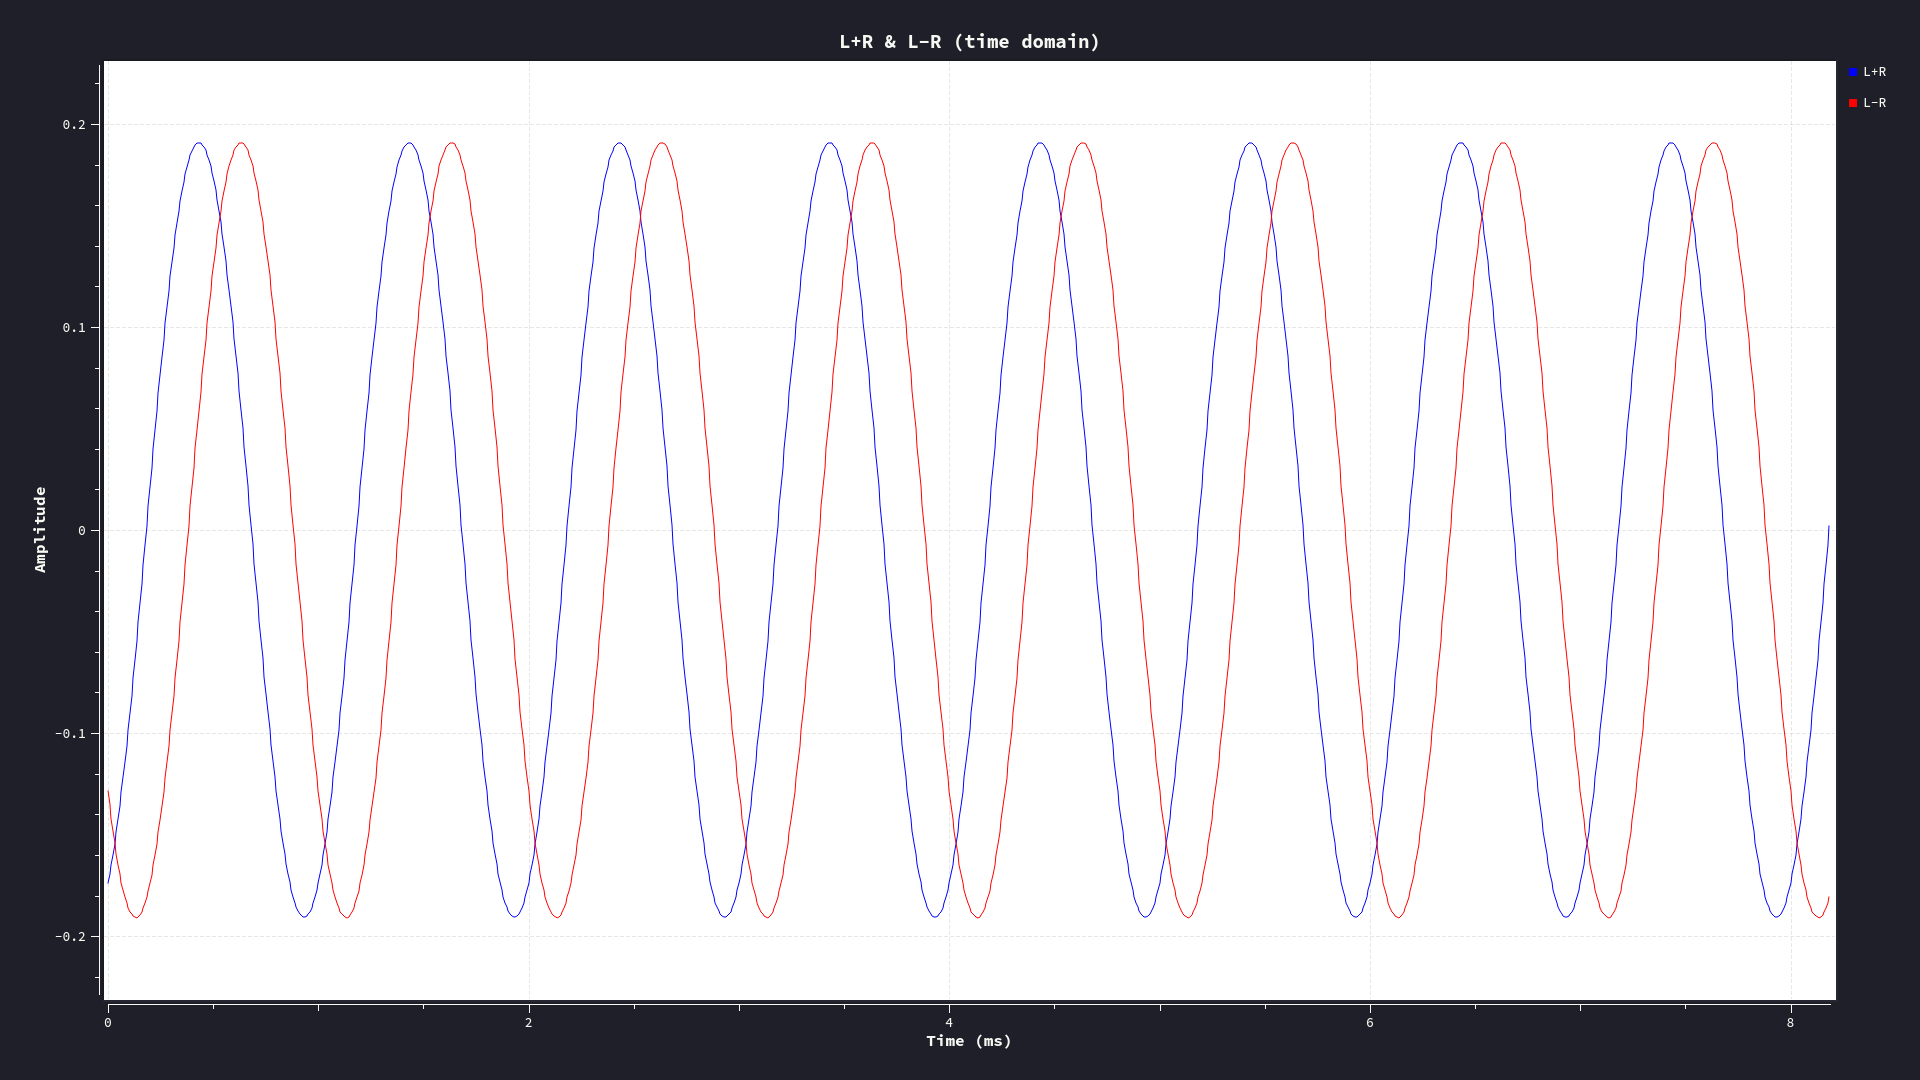
\includegraphics[width=0.9\linewidth]{img/peculiaridades/LEFT_sem_delay.png}
        \caption{LEFT: visualização de $L+R$ e $L-R$ sem \textit{delay}.} 
        \label{fig:a} 
        \vspace{4ex}
    \end{subfigure}%% 
    \begin{subfigure}[b]{0.5\linewidth}
        \centering
        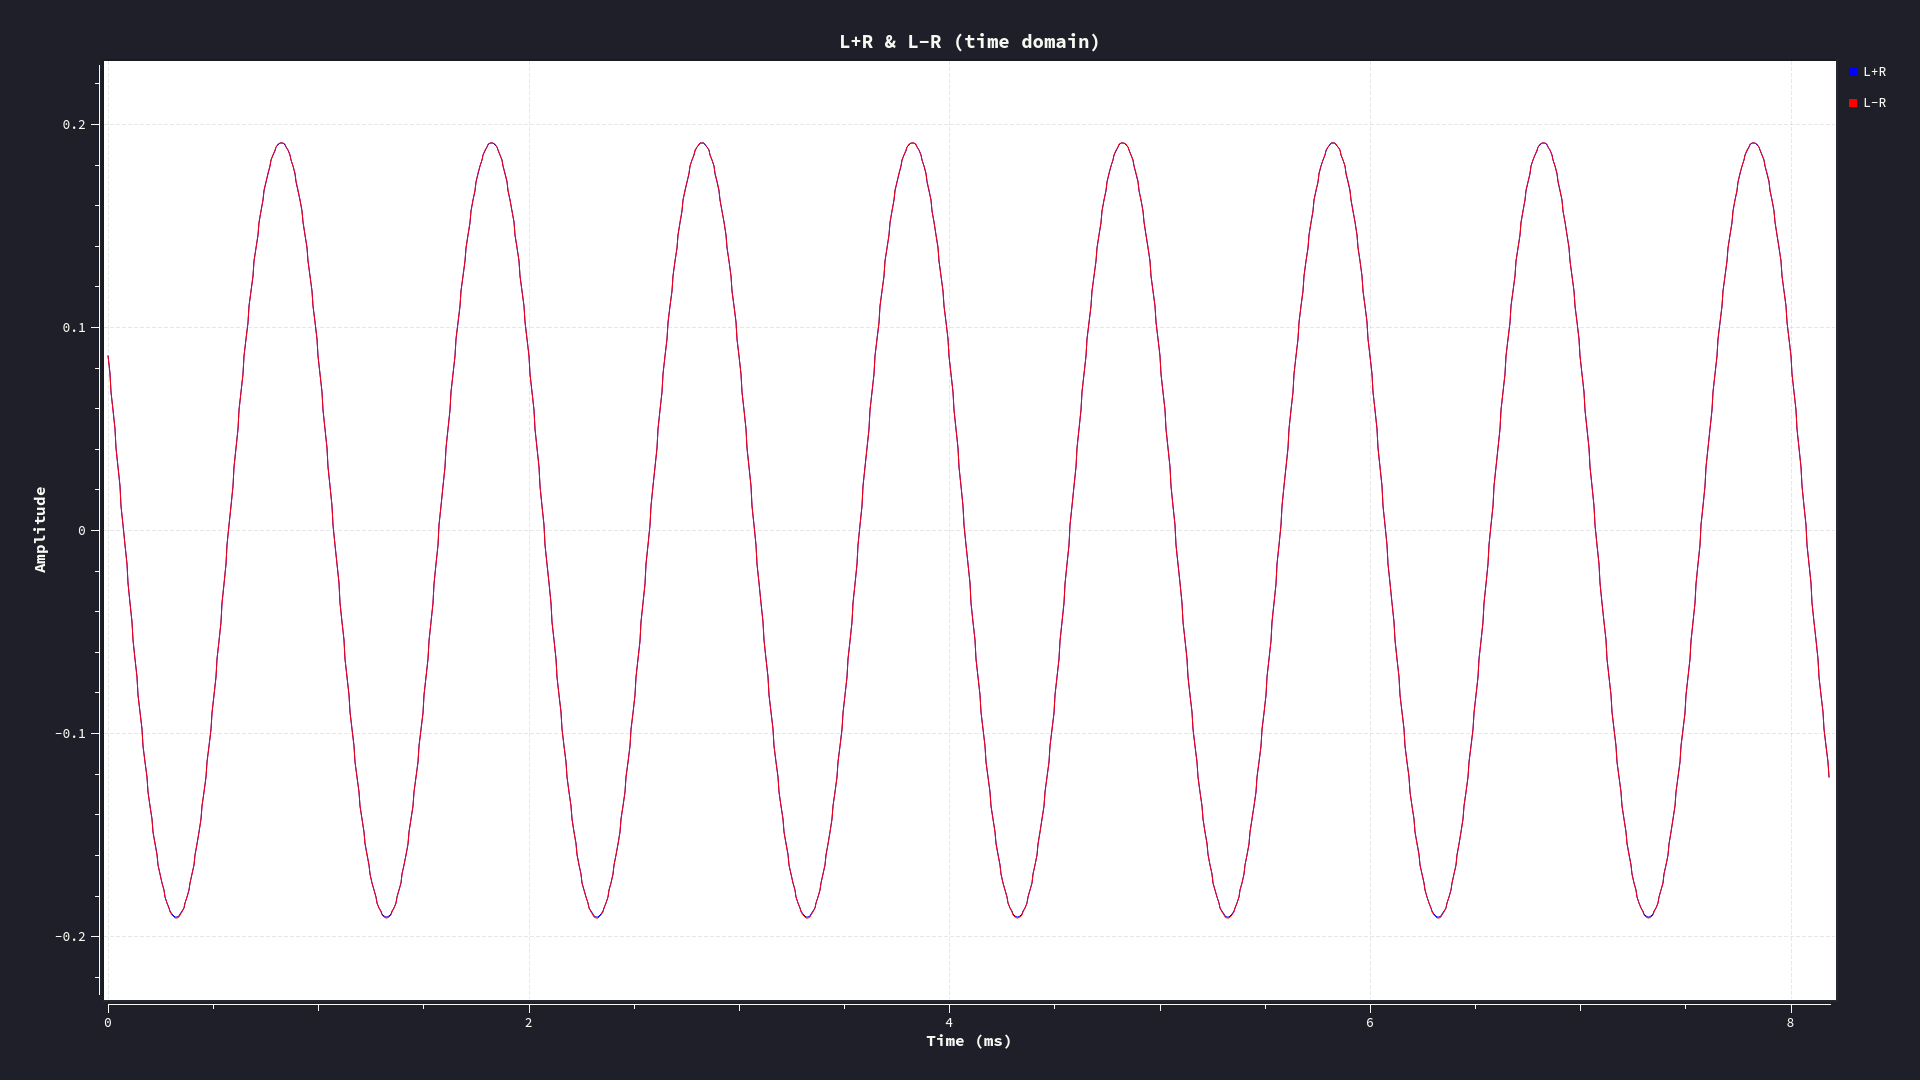
\includegraphics[width=0.9\linewidth]{img/peculiaridades/LEFT_com_delay.png} 
        \caption{LEFT: visualização de $L+R$ e $L-R$ com \textit{delay}.} 
        \label{fig:b} 
        \vspace{4ex}
    \end{subfigure} 
    \begin{subfigure}[b]{0.5\linewidth}
        \centering
        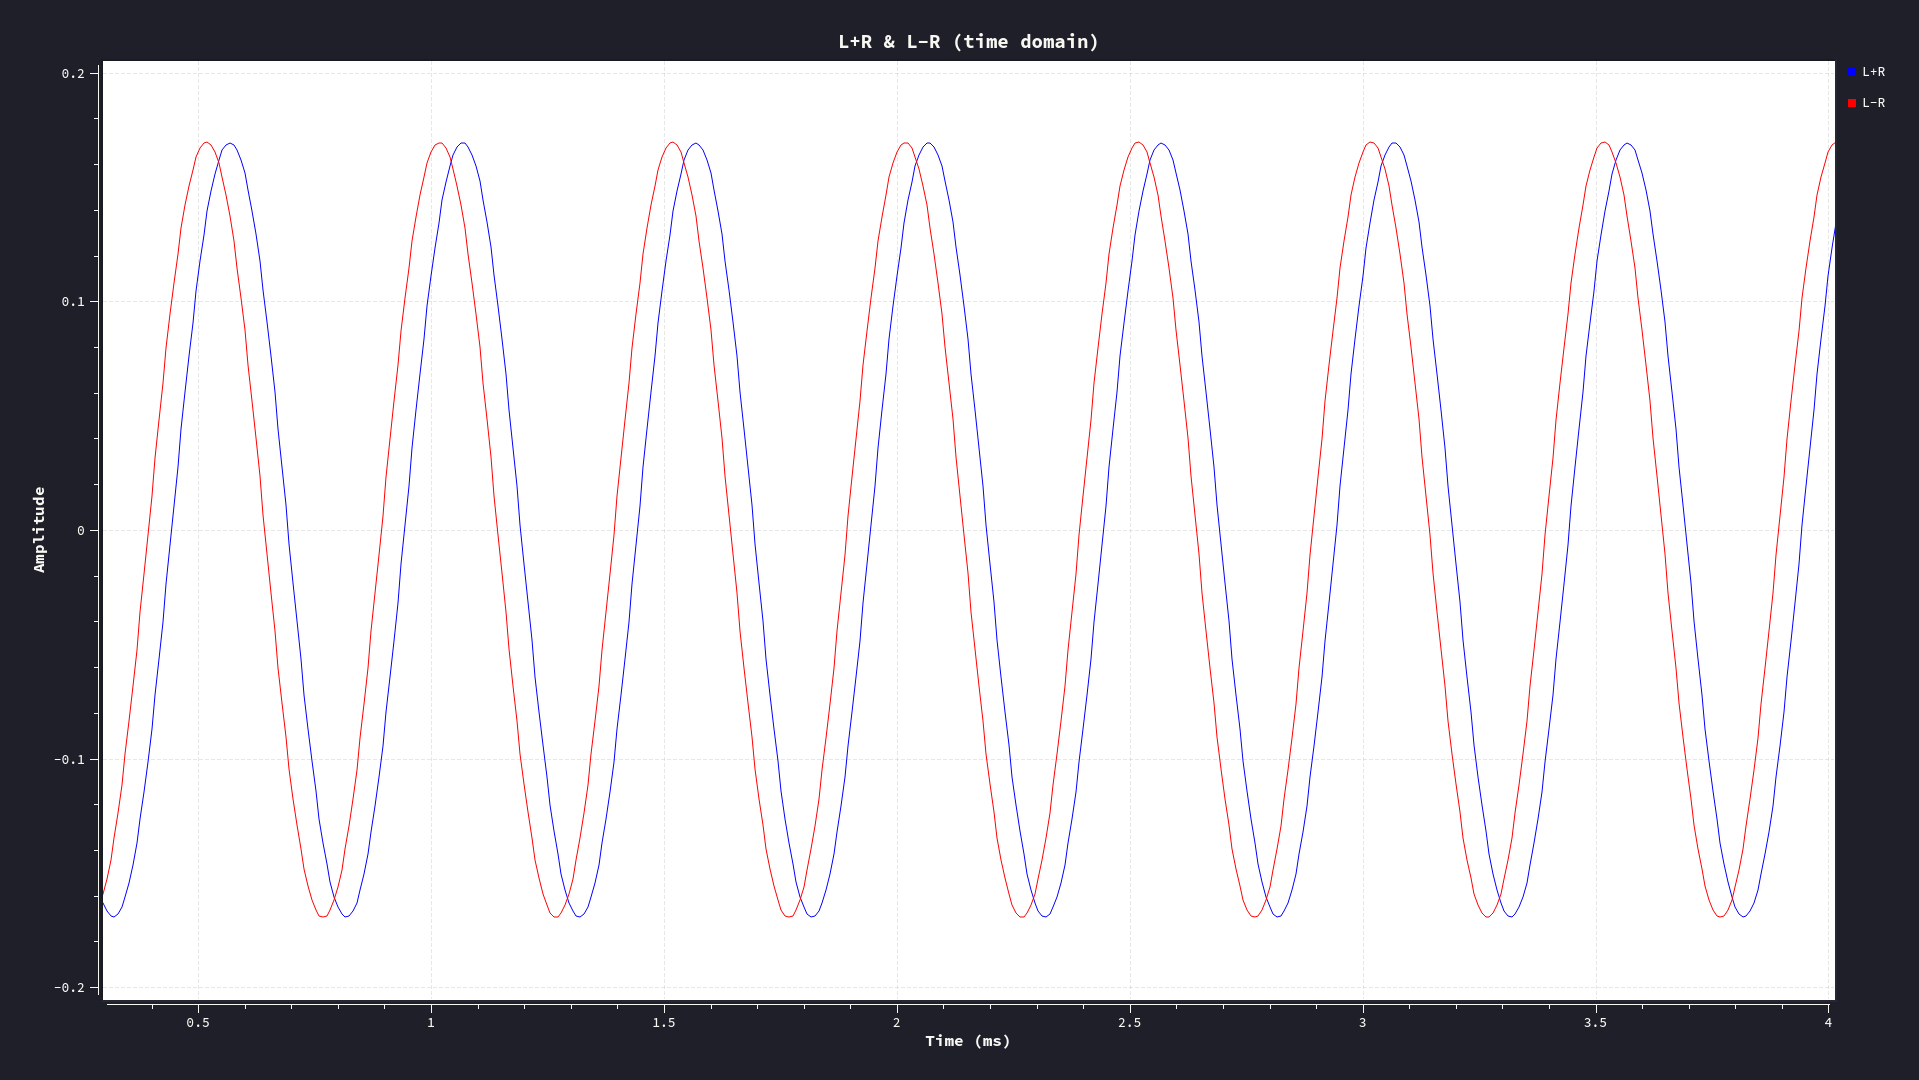
\includegraphics[width=0.9\linewidth]{img/peculiaridades/RIGHT_sem_delay.png}
        \caption{RIGHT: visualização de $L+R$ e $L-R$ sem \textit{delay}.} 
        \label{fig:c} 
        %%\vspace{4ex}
    \end{subfigure}%% 
    \begin{subfigure}[b]{0.5\linewidth}
        \centering
        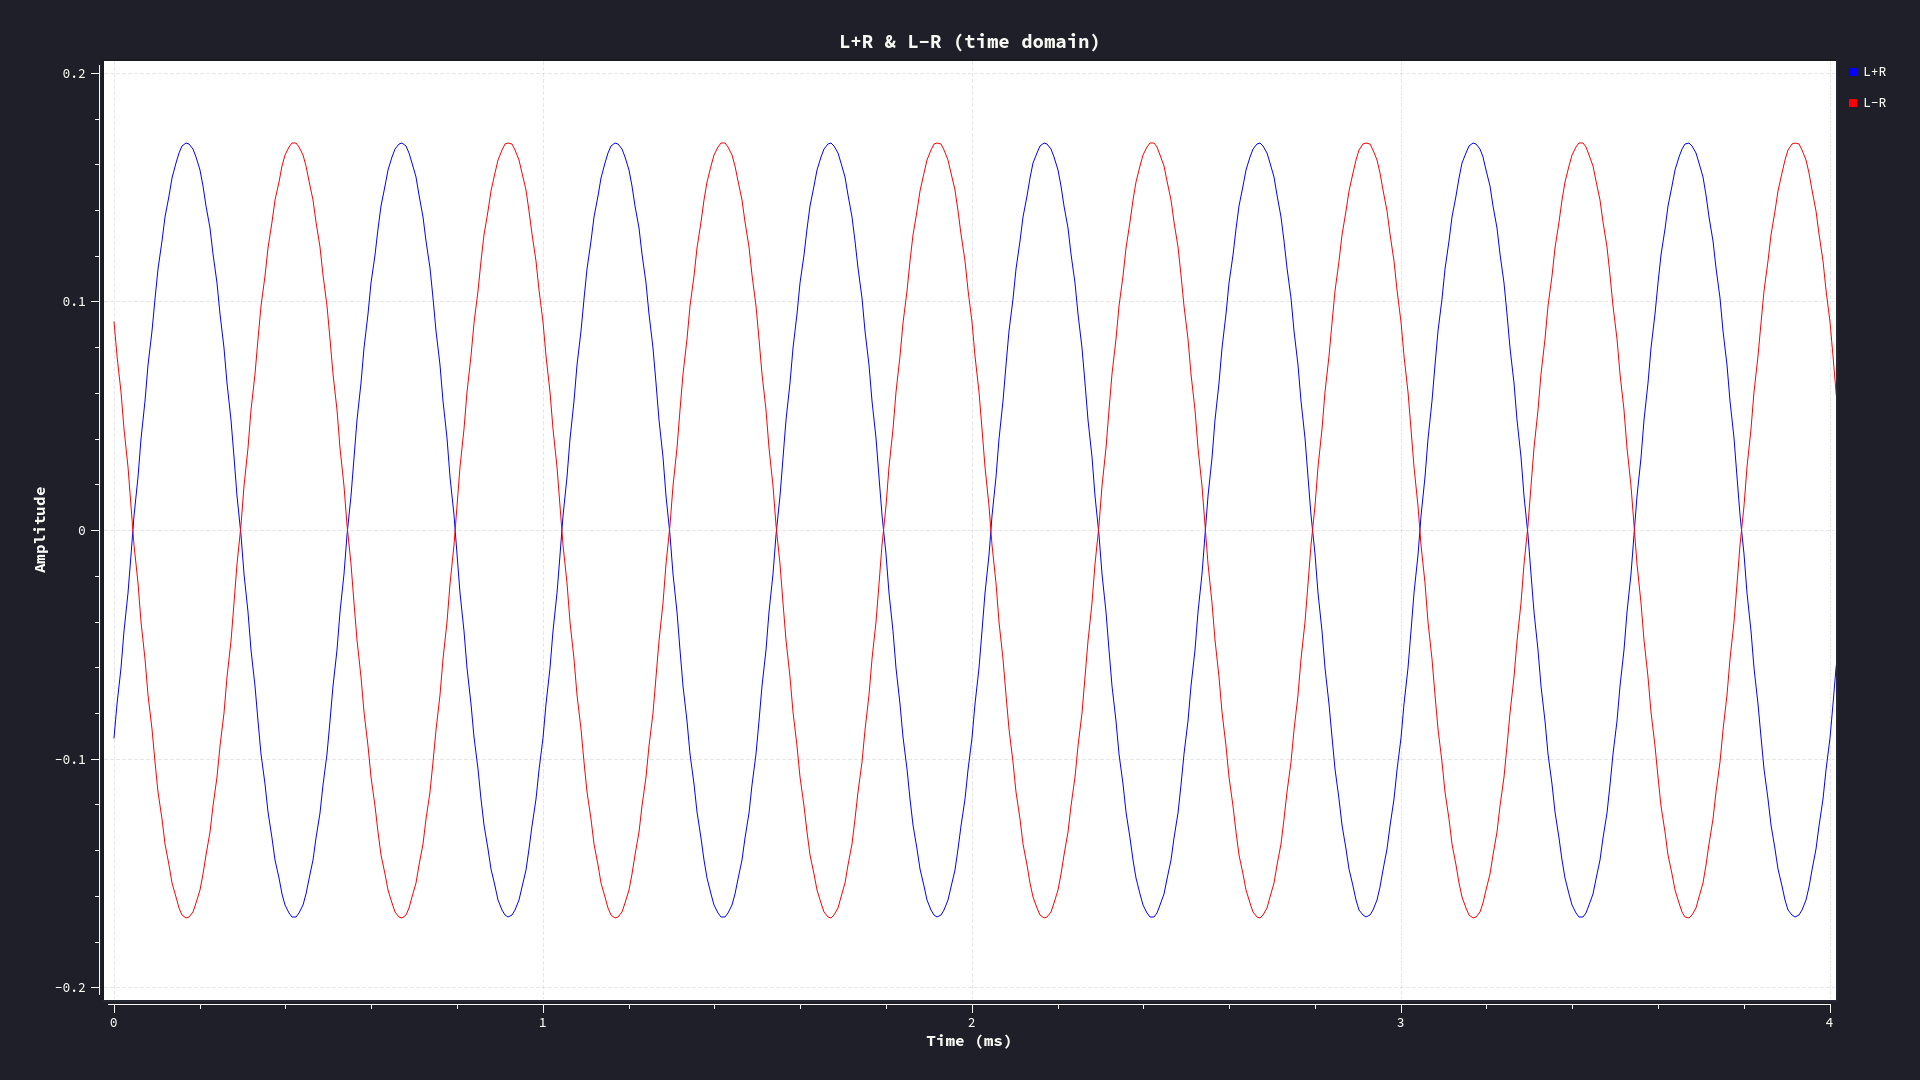
\includegraphics[width=0.9\linewidth]{img/peculiaridades/RIGHT_com_delay.png} 
        \caption{RIGHT: visualização de $L+R$ e $L-R$ com \textit{delay}.} 
        \label{fig:d} 
        %%\vspace{4ex}
    \end{subfigure} 
    \caption{Efeitos da calibração com o bloco de \textit{delay} no final do ramo que recupera $L+R$.}
    \label{fig:multiplas}
\end{figure}
%3
%3
%=============================--D--=============================%
\subsection{3. Filtros de de-ênfase}

%\iffalse
\begin{figure}[H]
    \centering
    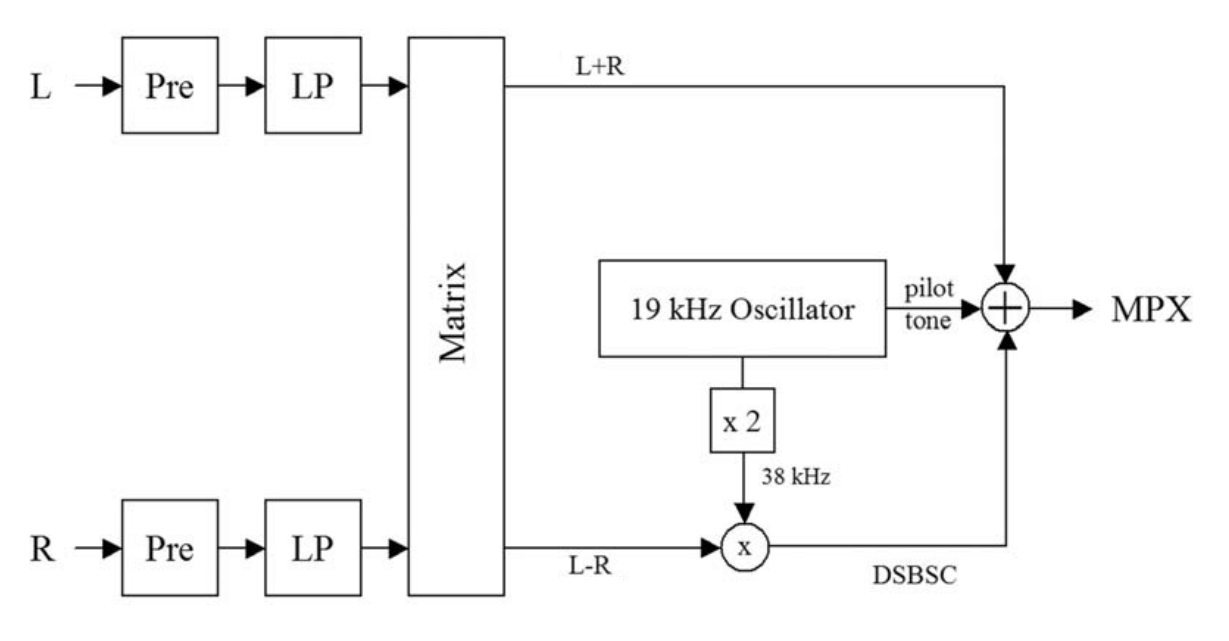
\includegraphics[width = 0.7\linewidth]{img/peculiaridades/encoder_stereo.png}
    \caption{Codificador stereo com filtros de pré-ênfase (Pre) e filtros passa-baixo (LP).}
    \label{fig:stereo_encoder}
\end{figure}
%\fi

No processo de codificação da mensagem, exposto na \hyperref[fig:stereo_encoder]{Fig. 5}, os sinais $L$ e $R$ são sujeitos a filtros de pré-ênfase com o intuito delineado na seguinte citação:

\textit{"Pre-emphasis (giving High frequencies a boost) is applied to both channels before the multiplexing process. A corresponding de-emphasis is applied at the receiver. The idea of this is to lift the high frequency signal some so that in the receiver you can reduce the high frequency ALONG WITH some of the hiss from the receiver. In Australia [NOTA: o mesmo para a Europa\cite{transmission_standards_for_fm_sound_broadcasting_at_vhf}] we use a $50\ \mu$s time constant network for pre-emphasis, in USA they use $75\ \mu$s."}\cite{anintroductiontofmmpx}

\vspace{1.0em}
Tendo em conta o supracitado e a seguinte \hyperref[fig:bb]{Fig. 6 (b)}, é trivialmente deduzida a localização dos filtros de de-ênfase (\hyperref[fig:aa]{Fig. 6 (a)}).

\begin{figure}[ht] 
    \begin{subfigure}[b]{0.5\linewidth}
        \centering
        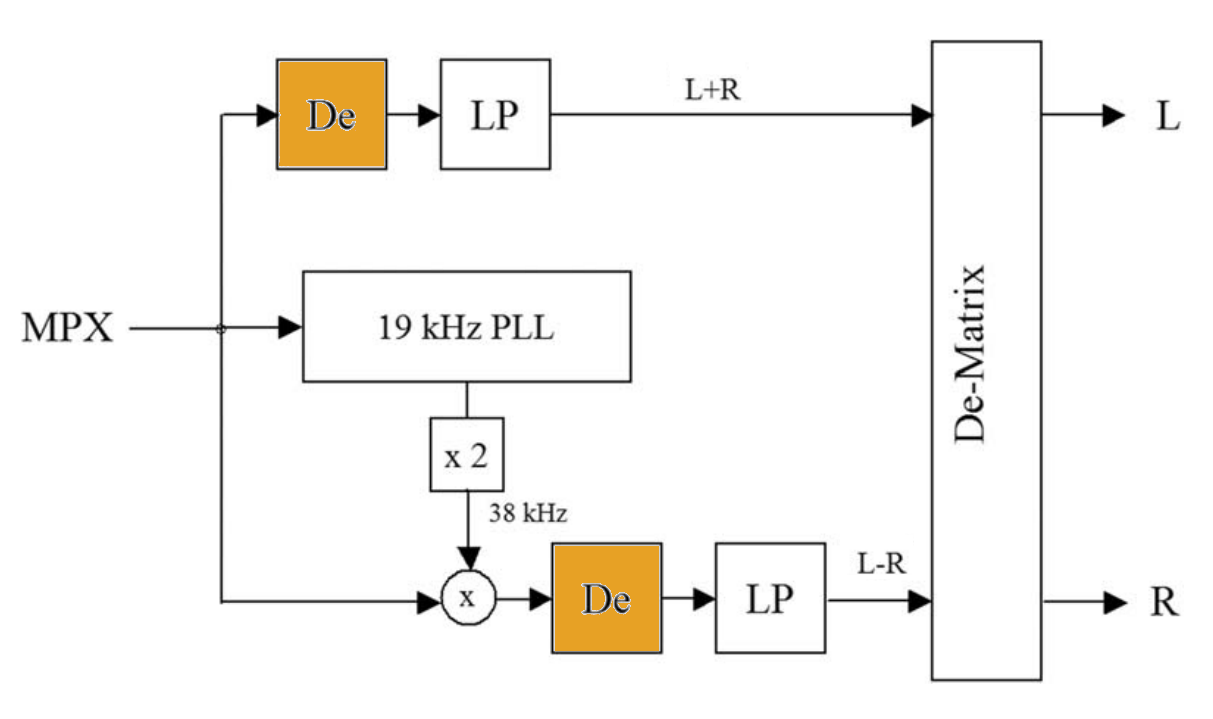
\includegraphics[width=0.90\linewidth]{img/peculiaridades/decoder_stereo.png}
        \caption{Descodificador stereo com \textcolor{orange}{filtros de de-ênfase (De)} \\ e filtros passa-baixo (LP).} 
        \label{fig:aa} 
        %\vspace{4ex}
    \end{subfigure}%% 
    \begin{subfigure}[b]{0.5\linewidth}
        \centering
        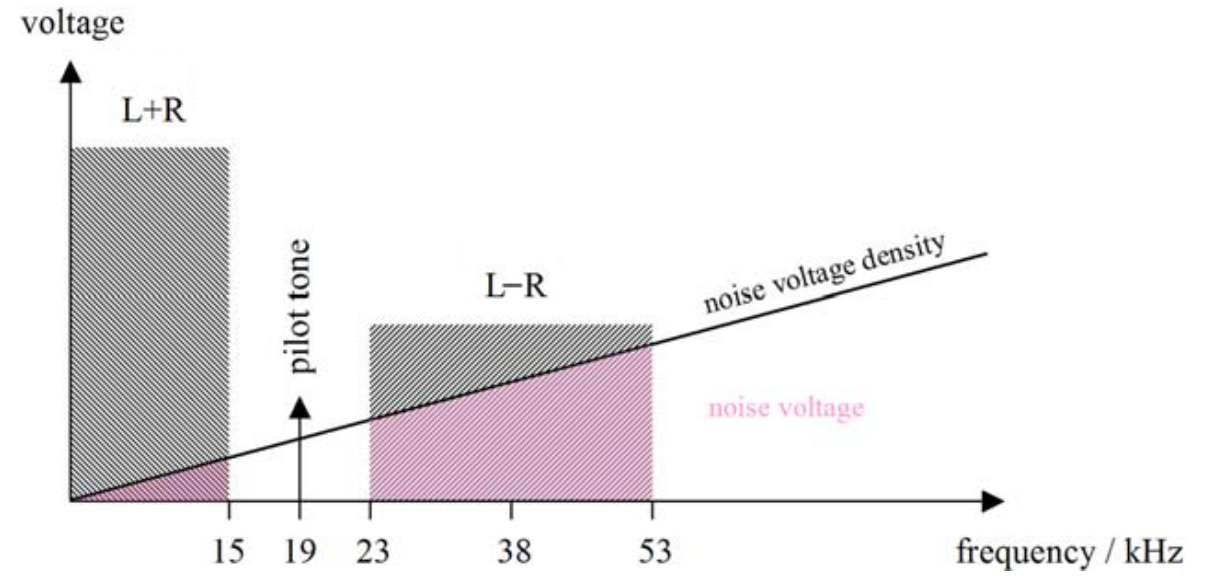
\includegraphics[width=0.90\linewidth]{img/peculiaridades/noise.png} 
        \caption{\textit{Noise voltage density} e \textit{\textcolor{pink}{noise voltage}}, sinais $L+R$ \\ e $L-R$.} 
        \label{fig:bb} 
        %\vspace{4ex}
    \end{subfigure} 
    \caption{De-ênfase.}
    \label{fig:multiplas2}
\end{figure}

O processo de de-ênfase efetua-se nos módulos \hyperref[subsec:mod2]{2} e \hyperref[subsec:mod3]{3} (antes dos filtros passa-baixo com $f_c = 15$ kHz), de modo a mitigar a \textit{noise voltage} das componentes $L+R$ e $L-R$. O resultado final traduz-se numa maior qualidade sonora à saída do \textit{dematrixer} (\hyperref[subsec:mod4]{módulo 4}).
\newline\break
\noindent\fcolorbox{black}{white}{%
    \minipage[t]{\dimexpr\linewidth-2\fboxsep-2\fboxrule\relax}
        \textbf{Observações} $\rightarrow$ A não utilização destes filtros supramencionados (no caso do sinal de teste IQ e transmissões rádio captadas pelo RTL-SDR), manifestou-se na presença audível de "som de estática" que deteriorou a qualidade sónora (o \textit{signal-to-noise ratio} é diminuído, perceptivelmente, com o aumento do ruído de fundo). A disposição destes blocos antes do "Audio Sink" resultou na redução de ruído de fundo, no entanto, este verificou-se \textit{muffled} (não ideal). A localização explicitada na \hyperref[fig:aa]{Fig. 6 (a)}, mostrou-se incrivelmente eficiente na redução do ruído audível, e não comprometeu a fidedignidade sonora.
    \endminipage}
